\section{Análisis de Arquitecturas de Antena}

\subsection{4.1 Antenas conformes para CubeSat}

Aunque los diseños tradicionales de antenas satelitales priorizaban estructuras rígidas, las plataformas CubeSat exigen soluciones que se adapten a superficies curvas y limitaciones volumétricas estrictas. Particularmente llamativo es el hecho de que las antenas conformes han surgido como alternativa prometedora precisamente por su capacidad de integrarse directamente sobre la estructura del satélite sin comprometer el espacio disponible para otras cargas útiles.

Guler et al. demuestran el potencial de phased-array conformes en escenarios LEO dinámicos, donde el escaneo electrónico permite mantener el enlace a pesar de los rápidos cambios de orientación y velocidad relativa \cite{Guler2025}. En muchos casos estudiados, estas configuraciones logran un compromiso aceptable entre ganancia y cobertura hemisférica, aunque tienden a sufrir degradación en eficiencia cuando se implementan sobre sustratos flexibles o con curvaturas pronunciadas. No obstante, cabe matizar que su bajo perfil y capacidad de beamforming adaptativo las hacen especialmente adecuadas para constelaciones dedicadas al monitoreo ambiental.

Resulta revelador observar cómo esta adaptabilidad estructural abre puertas a despliegues donde múltiples sensores y antenas comparten la misma plataforma sin interferencias mecánicas.

\subsection{4.2 Diseños de ganancia alta desplegables}

Uno de los desafíos persistentes al dimensionar enlaces uplink desde sensores de muy bajo consumo radica en la necesidad de ganancia elevada desde el segmento espacial. Lejos de ser un asunto resuelto, las antenas helicoidales desplegables ofrecen una ruta práctica para alcanzar ganancias superiores a 10 dBi manteniendo peso mínimo.

Meirambekuly et al. presentan un diseño helicoidal cónico L/S integrado con sistema óptico para CubeSats de observación terrestre, destacando excelente rendimiento en despliegue, polarización circular y estabilidad en órbita \cite{Meirambekuly2023}. Estos sistemas tienden a superar a las soluciones fijas en escenarios donde se requiere haz estrecho y alta directividad. Aun así, sacrifican flexibilidad de escaneo, lo que obliga a complementar con mecanismos de control de actitud del satélite.

En comparación directa con arquitecturas conformes, los diseños desplegables destacan en aplicaciones que priorizan margen de enlace sobre agilidad de haz, un trade-off crítico en redes de sensores ambientales dispersos.

\begin{table*}[htbp]
\renewcommand{\arraystretch}{1.5} % Mantiene el espaciado vertical estandarizado por la IEEE
\centering
\caption{\textsc{Métricas de Ganancia y Rendimiento Comparadas para Arquitecturas L/S en Plataformas LEO}}
\label{tab:metricas_antenas_leo}
% \columnwidth obliga a la tabla a medir exactamente el ancho del margen de la columna actual
\begin{tabularx}{\columnwidth}{|X|c|c|c|c|}
\hline
\textbf{Arquitectura} & \textbf{Banda} & \textbf{Ganancia} & \textbf{Eficiencia} & \textbf{Beamwidth} \\
\textbf{} & \textbf{} & \textbf{Máx. (dBi)} & \textbf{(\%)} & \textbf{($^{\circ}$)} \\ \hline
Conforme Phased-array & L & 8–12 & 65–75 & 60–90 \\ \hline
Helicoidal desplegable & S & 12–15 & 70–80 & 30–45 \\ \hline
Patch multibanda & L/S & 7–11 & 55–70 & 70–100 \\ \hline
Phased-array multibanda & S & 10–14 & 60–78 & Variable \\ \hline
\end{tabularx}
\end{table*}

\subsection{4.3 Phased-array multibanda}

Resulta especialmente interesante cómo la evolución hacia arrays multibanda busca resolver simultáneamente restricciones de masa y espectro. Roy et al. exploran antenas de estación terrestre dual-band S-X que, aunque orientadas al segmento ground, ofrecen lecciones valiosas sobre manejo de acoplamiento y patrones de radiación que pueden contrastarse con soluciones espaciales \cite{Roy2022}.

En el contexto espacial, los phased-array multibanda tienden a proporcionar mayor flexibilidad operativa, permitiendo conmutación dinámica entre bandas L y S según condiciones de propagación o requisitos del sensor. Sin embargo, la complejidad del alimentador y los desafíos de aislamiento entre bandas introducen pérdidas adicionales que deben compensarse cuidadosamente en el link budget.

Lejos de constituir una solución universal, estas arquitecturas destacan en escenarios donde se requiere reconfigurabilidad elevada. Su integración con algoritmos de beamforming adaptativo podría mitigar algunos de los efectos Doppler discutidos previamente, aunque aumenta el consumo energético a bordo —un factor limitante en CubeSats de bajo presupuesto.

\begin{figure}[h]
\centering
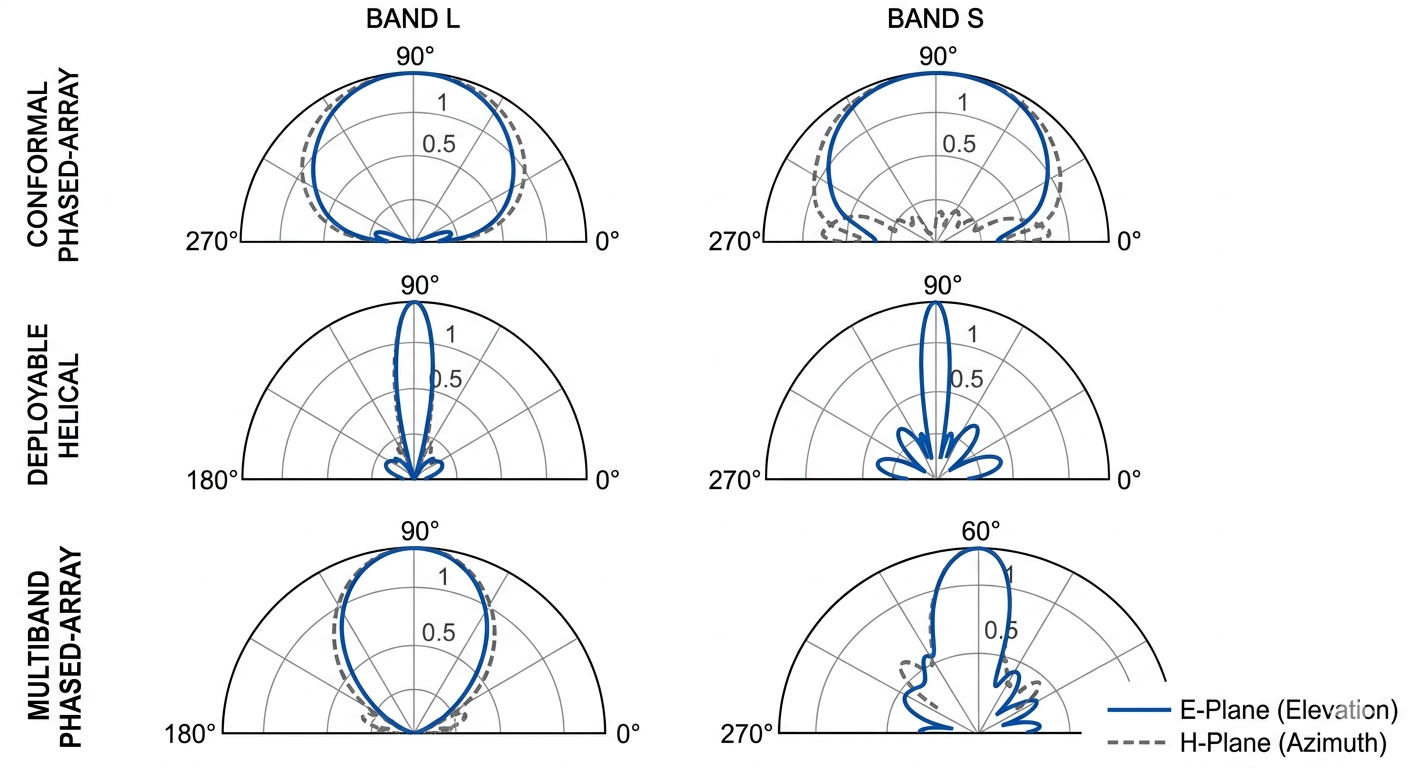
\includegraphics[width=\linewidth]{fig3.png}
\caption{Diagramas de radiación normalizados en bandas L y S para las tres arquitecturas principales analizadas: phased-array conforme, helicoidal desplegable y multibanda, mostrando patrones en planos azimutal y de elevación.}
\label{fig:radiation_patterns}
\end{figure}

El análisis comparativo revela que ninguna arquitectura domina universalmente. La selección óptima dependerá de los requisitos específicos de la misión ambiental: cobertura amplia versus ganancia elevada, consumo versus reconfigurabilidad. Estas consideraciones guían la evaluación cuantitativa presentada en la siguiente sección.